\chapter{Referencial Teórico}
\label{chap:Ref}
	Neste capítulo serão apresentados os conceitos utilizados na pesquisa, bem como
	os estudos que fundamentaram esse projeto. A Seção \ref{sec:Mooc} apresenta
	o conceito de MOOC e as principais características da plataforma de ensino.
	A Seção \ref{sec:MinVisual} descreverá  A
	Seção \ref{sec:FundTeor} descreve as definições de termos presentes no decorrer
	da pesquisa. A Seção \ref{sec:TrabRel} apresenta as pesquisas relacionados a
	este estudo juntamente com suas limitações.

	\section{Massive Open Online Courses (MOOC)}
	\label{sec:Mooc}
		Após pesquisar o conceito de Curso Massivo, Aberto e \foreign{Online},
		\citeonline{fassbinder2014} observam que não há uma definição comum na
		literatura. Entretanto, encontra três descrições distintas para o termo.
		Enquanto \citeonline{sivamuni2013} afirma que o MOOC, em conformidade com
		o dicionário Oxford, é um curso oferecido por meio da Internet, de forma
		gratuita, para uma grande quantidade de alunos. \citeonline{subbian2013}
		reitera que o MOOC disponibiliza curso gratuito, baseado na \foreign{web},
		com registro livre de taxas monetárias e compartilhamento público de
		currículo. \citeonline{siemens2013} defende a tendência em inovação e
		experimentação do uso da tecnologia para o ensino a distância e
		\foreign{online} a fim de dar oportunidade de aprendizagem de forma massiva.
		
		\citeonline{kim2014} afirma que massivo refere-se a capacidade do MOOC em
		suportar uma grande quantidade de alunos. Tal quantidade é bem superior
		ao número de discentes que uma sala pode acomodar ou o total de
		participantes em um curso \foreign{online} antes do surgimento do MOOC.
		Por exemplo, um curso de Inteligência Artificial foi ofertado, gratuitamente e
		\foreign{online}, pela Universidade de Stanford em 2011, no qual houveram
		160.000 estudantes inscritos \cite{rodriguez2012}.
		
		Entre os principais recursos da plataforma, como a integração com outras
		aplicações (e-mails), o uso de questionário relacionados com os vídeos e a
		inclusão de atividades para estimular e motivar os alunos \cite{fassbinder2014}.
		Focaremos no desenvolvimento de recursos avançados de visualização dos dados
		obtidos por meio das implementações submetidos em cursos de programação e
		na realização de \foreign{feedback} para que o usuário possa verificar seu nível
		de conhecimento.

	\section{Fundamentação Teórica}
	\label{sec:FundTeor}
		Nesta seção apresentaremos as definições de alguns termos utilizados
		durante a pesquisa: mineração e visualização de dados, projeção e a diferença
		na área de Inteligência Artificial sobre classificadores e agrupamento.
		
		A mineração de dados é uma etapa do \foreign{Knowledge Discovery in Databases}
		\cite{fayyad1996} que busca descobrir padrões em grandes conjuntos de dados
		podendo utilizar métodos de inteligência artificial, estatísticos e sistemas
		de banco de dados \cite{chakrabarti2006}. O objeto do processo de mineração
		de dados consiste na extração de informações de um conjunto de dados e
		transformá-lo em uma estrutura compreensível para uso posterior \cite{chakrabarti2006}.
		Muitos métodos de mineração de dados são baseados em técnicas de treinamento
		e teste de aprendizagem de máquina, reconhecimento de padrões e estatísticas,
		como os algoritmos de classificação e agrupamentos \cite{fayyad1996}.
		
		\textbf{No artigo \cite{fayyad1996} há um fluxograma do KDD (Figura 1).
		Quando fui pesquisar na internet sobre um fluxograma de mineração, apareceram
		vários fluxogramas iguais! Não coloquei porque fiquei na dúvida. Posso utilizar
		o fluxograma do KDD pra exemplificar a mineração de dados?}
		
		Após a mineração das informações, é necessário a utilização de ferramentas
		para criar hipóteses sobre conjuntos de dados complexos -- grande conjunto
		de dados ou de alta dimensionalidade -- para que os analistas possuam
		capacidade de explorá-los e compreendê-los. A visualização de dados produz
		modelos gráficos e representações visuais a fim de utilizar a capacidade
		cognitiva do ser humano, por meio da percepção visual, para colaborar com
		a exploração e obtenção de informações úteis presente nos dados \cite{de2003}.
		
		\textbf{O parágrafo acima foi inteiramente retirado da referência. Cito só
			no final do parágrafo ou ao final de cada frase? No parágrafo abaixo
			ocorre o mesmo problema de citação. De "Entretanto os modelos..."
			até "tridimensional." é tudo do mesmo artigo.}
		 
		Para exibir visualizações geradas a partir da mineração de dados de
		baixas dimensões, foi criado o mapeamento de dados para reconhecimento
		visual, chamado de projeção \cite{friedman1974}. Entretanto os modelos gráficos
		ou as representações visuais podem possuir alta dimensão devido ao grande
		conjunto da base de dados e de características extraídas. Por consequência,
		há uma dificuldade para que a visualização seja representada em um plano de
		baixa dimensão. Para isso, criou-se uma técnica de projeção: projeção
		multidimensional. Essa técnica realiza a diminuição $n-dimensional$, sendo
		$n$ uma alta dimensão, para uma espaço unidimensional, bidimensional ou
		tridimensional \cite{paulovich2008least}. Para criar essa visualização
		deve-se selecionar o formato de como as características extraídas serão
		armazenadas, como o vetor de características ou o modelo de tabela de dados
		\cite{de2003}.
		
		Classificação é a tarefa de aprendizagem de uma função alvo que mapeia cada
		conjunto de atributo a um dos rótulos de classe predefinidas \cite{Tan:2005:ch4}.
		Uma função alvo auxilia como uma ferramenta que possui informações para distinguir
		os objetos de diferentes classes. A fim de realizar essas classificações, são
		implementados classificadores com diversas abordagens, como árvore de decisão,
		redes neurais e \foreign{support vector machine}, por exemplo. Esses
		classificadores são mais utilizados para predizer ou descrever um conjunto
		de dados com categorias binárias ou nominais. Por exemplo, para classificar
		um animal como mamífero, réptil, peixe, anfíbio ou pássaro, deve-se sumarizar
		dados como a temperatura do corpo, característica da pele, se é uma criatura
		aquática, se possui patas e hiberna.
		
		O que difere a classificação do agrupamento, é que esse é formado por meio da
		comparação de informações entre os objetos, enquanto aquele é realizado por meio
		da comparação das informações do objeto com os dados contidos na função alvo.
		Desta forma, os objetos dentro de um grupo devem ser similares ou relacionados
		entre si e, diferentes ou não relacionados entre objetos de grupos diferentes,
		ou seja, quanto maior a similaridade dos objetos dentro de um grupo e mais
		diferentes são os agrupamentos, melhor ou mais distinto os agrupamentos
		\cite{Tan:2005:ch8}. O K-means \cite{macqueen1967} e o \foreign{Density-based
		Algorithm for Discovering Clusters} \cite{Ester1996} são exemplos de algoritmos
		de agrupamento.

	\section{Mineração e Visualização de Programas}
	\label{sec:MinVisual}
		Para realizar a mineração de informações nos programas submetidos, é necessário
		decidir como será extraído as características -- análise sintática, dinâmica e
		do código de escrita -- e quais dados podem ser obtidos por meio da análise
		escolhida (Subseção \ref{subSec:Caracteristicas}). Independente da dimensão
		obtida por meio da quantidade de informações extraídas, é necessário escolher
		como os dados obtidos serão armazenados para que seja possível realizar sua visualização.
		
		\subsection{Características de Programas}
		\label{subSec:Caracteristicas}

			A extração de características por meio das implementações podem ocorrer das
			seguintes formas: análise estática, análise dinâmica e análise do estilo de escrita.
			A análise estática ocorre por meio da observação do código-fonte, considerando
			apenas sua implementação, ou seja, não é necessário sua execução. Há diversas
			características que podem ser extraídas dessa análise. Há abordagens que extraem
			somente a Árvore de Sintaxe Abstrata (AST) que pode ser gerada durante a análise
			sintática do compilador para representar o código-fonte em forma de árvore
			armazenando símbolos não-terminais nos nós filhos e símbolos terminais nos
			nós folha. Esse tipo de árvore possui símbolos não terminais como nós filhos
			e símbolos terminais como nós folhas. Enquanto outras abordagens extraem
			características como: a quantidade de linhas e atribuições da implementação,
			a complexidade ciclomática \cite{mccabe}, quantidade de variáveis, operadores,
			operandos, laços de repetição e laços de repetição aninhados, por exemplo.
			
			A análise dinâmica do código-fonte consiste na observação da execução do
			programa, por meio do \foreign{trace} -- uma espécie de histórico de execução
			do programa -- e de teste de \foreign{software}. Analisando esse histórico é
			possível verificar algumas características, como: em que momento foi realizado
			uma atribuição, chamada de função e recursão, qual bloco de código foi
			executado em uma declaração de condição, a quantidade de vezes que um laço
			de repetição foi executado e a saída no final da execução. Já o teste de
			software pode ser utilizado executando casos de teste em que verifica se a
			produção final do programa era o esperado e esta informação, se o caso de
			teste funcionou corretamente ou não, também pode ser uma característica do programa.
			
			E a análise do estilo de escrita, que será utilizada no desenvolvimento desse projeto,
			é um tipo da análise estática. Entretanto, se difere no fato das implementações estarem
			sintaticamente corretas. Nesse tipo de análise é considerado o estilo de escrita do
			programador, abrindo a possibilidade de coletar dado estáticos, como a quantidade de
			linhas de código e sua complexidade. Além da possibilidade de coletar
			características da análise estática citada anteriormente, é possível coletar se:
			há mais que uma instrução e importação de bibliotecas por linha, há espaços entre
			operando e operador, os métodos são separados por uma linha em branco e tamanho
			da instrução, medido em caracteres.
			
			\begin{table}
				\centering
				\begin{tabular}{|c|c|}
					\hline
					Chamada de função & Instrução por linha \\ \hline
					primo(7)          & a = 5 * 3  \\
					primo( 7)         & primo(7)     \\
					primo(7 )         &      \\
					primo( 7 )        & a = 5 * 3; primo(7)    \\
					\hline
				\end{tabular}
				\captionsetup{justification=centering}
				\caption[Representação do estilo de escrita]{Representação do estilo
				de escrita pode ocorrer com variações de espaços e mais que uma
				instrução por linha, por exemplo.}
			\end{table}
			
			Além da possibilidade de extrair os dados citados anteriormente. É possível
			obter os dados de como foi realizado o processo técnico e social do desenvolvimento
			do programa. Para ambas abordagens, é necessário a utilização de um sistema de
			controle de versão para que possa utilizar seus recursos. Um mecanismo para
			obter informações é em relação ao momento, data e hora, em que o aluno realizou
			um \foreign{commit} de uma versão da sua implementação. Outro método é verificar
			se houve comunicações com outras pessoas durante o desenvolvimento do programa,
			por meio da interação em \foreign{issues} ou solicitações de \foreign{pull requests}.
			
			\textbf{Eu não entendi a seguinte inserção nessa subseção que você solicitou:
				"Problema (atividade de aprendizagem sendo elaborada)"}

	\section{Trabalhos Relacionados}
	\label{sec:TrabRel}
	
	    A fim de encontrar a semelhança entre os códigos, \citeonline{Yin:2015}
	    utilizou a AST. Após a criação das árvores, é necessário o uso de métricas
	    para verificar a similaridade entre as árvores. Desta forma, foi utilizada
	    a Distância de Edição de Árvore (TED) – ao comparar duas árvores, verificam-se
	    quais são as movimentações (inserção, movimentação e remoção) necessárias
	    para que as árvores fiquem iguais. Assim, foi selecionado a TED normalizado
	    que utiliza estrutura \foreign{top-down}: quanto mais próximo do nó raiz,
	    maior sua importância. Sua escolha ocorreu pelo fato do TED normalizado
	    possuir maior índice na qualidade de agrupamentos.
	    
	    Os autores desse artigo analisado utilizaram os algoritmos de agrupamento
	    DBSCAN \cite{Ester1996} e OPTICS \cite{Ankerst1999} para agrupar os códigos
	    semelhantes, visto que esses algoritmos de agrupamento obtiveram a maior
	    pontuação de silhueta que verifica a similaridade entre pares dentro do
	    agrupamento e entre os agrupamentos. Quanto maior sua pontuação, melhor a
	    qualidade do \foreign{cluster}. Conforme a Figura \ref{fig:t-SNE}, para
	    visualizar os agrupamentos foi utilizado o t-SNE \cite{maaten2008} – técnica
	    utilizada para reduzir dados de alta dimensionalidade para duas ou três
	    dimensões preservando a estrutura local dos dados.
	    
	    \begin{figure}[ht]
	        \centering
	        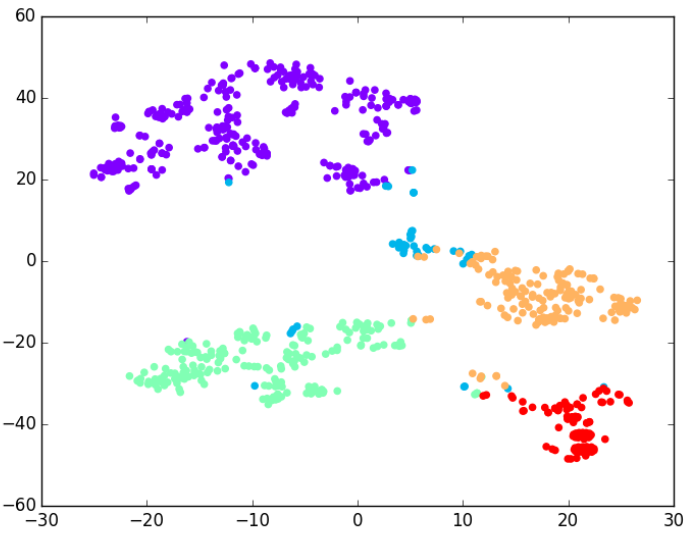
\includegraphics[scale=0.5]{imagem/visualizacao-tSNE.png}
	        \captionsetup{justification=centering}
	        \caption{Visualização t-SNE.}
	        \label{fig:t-SNE}
	    \end{figure}
	    
	    \textbf{Professora, na primeira revisão você questionou o que a função
	    	combine\_anagrams faz. Entretanto, revisei o artigo e não é realizado
	    	nenhuma menção ao objetivo da função. Devo tirar o nome da função? E
	    	a figura citada abaixo estava aqui! rs}
	    
	    Na Figura \ref{fig:t-SNE} é possível observar cinco grupos distintos
	    criados a partir da comparação das TEDs normalizadas: roxo, verde, laranja,
	    vermelho e azul. Cada ponto presente na visualização corresponde a uma
	    implementação. Todas as implementações possuem a função \foreign{combine\_anagrams}
	    que possui a variável \foreign{words} como parâmetro: no grupo vermelho,
	    essa função possui 3,7 linhas; no agrupamento roxo, 10,9 linhas; no
	    grupo laranja, a função possui 12,5 linhas; e no agrupamento verde,
	    a solução possui 21,3 linhas. Enquanto os pontos azuis não obtiveram
	    similaridade suficiente para formar um agrupamento ou serem classificados
	    em outro agrupamento. 

		A utilização da extração de características por meio da AST é interessante,
		como também o uso da TED normalizada para verificar sua similaridade, devido
		ao seu baixo custo computacional. Entretanto, como o autor testou seu
		agrupamento somente com implementações para resolver um problema, não sabemos
		se tal abordagem é eficiente quando houver implementações que buscam resolver
		diversos problemas. Em razão da possibilidade dos códigos-fontes gerarem
		árvores parecidas ainda quando solucionam problemas distintos.
	    
	    Em \citeonline{Glassman:2014}, foi proposto um agrupamento hierárquico de dois
	    níveis. No nível mais alto ocorre o particionamento das soluções ao longo do
	    plano de separação, considerando apenas características abstratas, como:
	    posição da declaração de condicional em relação a declarações de laço de
	    repetição (antes, dentro ou depois), profundidade de um laço de repetição
	    (\foreign{loop}) aninhado, números de nós AST e declarações de retorno,
	    \foreign{loops} e comparações, por exemplo.
	    
	    Dentro de cada agrupamento de alto nível, tem um subagrupamento, destinado a
	    capturar a dimensão generalizada, construções de linguagem de baixo nível e
	    bibliotecas utilizadas. Os agrupamentos internos são formados por meio de 48
	    características concretas: operações aritméticas e lógicas, laços de repetição,
	    funções de bibliotecas, declarações de atribuição, \foreign{loops}, condicional,
	    número de variáveis e valores constantes, por exemplo.
	    
	    \citeonline{Glassman:2014} utiliza o algoritmo de agrupamento \foreign{K-means}
	    para agrupar as implementações dos estudante. Foi utilizado diversos valores para $k$
	    e a validação dos agrupamentos ocorreu por meio da comparação dos \foreign{clusters}
	    criado pelo algoritmo de classificação com o que foi criado pelos professores.
	    Para os TAs foi entregue 50 códigos  dos estudantes randomicamente e notou-se
	    que eles ignoraram características de baixo nível.
	    
	    Estes utilizaram a métrica Informação Mútua Ajustada (AMI, do inglês
	    \foreign{Adjusted Mutual Information}), cálculo probabilístico, para comparar
	    os agrupamentos dos TA's com cada agrupamento gerado pelo \foreign{k-means}.
	    Quando o valor de AMI é 0 (zero), quer dizer que os agrupamentos são
	    independentes, entretanto, se for igual a 1, indica perfeita concordância
	    entre os \foreign{clusters}. Quando $k$ tinha um valor maior ou igual a 15,
	    os agrupamentos concordaram com o agrupamento de cada professor, conforme
	    medição do AMI.
	    
	    Apesar da grande quantidade de dados extraídos das implementações, não houve
	    nenhum alusão sobre como essas características interfeririam na cálculo de
	    similaridade utilizado. Contudo a abordagem de dividir as informações a serem
	    coletadas em duas dimensões é relevante. Posto que as implementações com
	    a mesma quantidade de laços de repetição, por exemplo, deveriam ser agrupadas
	    facilitando a verificação se os alunos entenderam como fazer e utilizar
	    tal instrução.
	    
	    Em \citeonline{Taherkhani:2012}, testou-se a ferramenta Aari para cinco tipos
	    de métodos de ordenação: \foreign{bubble sort}, \foreign{insertion sort},
	    \foreign{selection sort}, \foreign{mergesort} e \foreign{quicksort}. Os autores
		separaram as características em quatro categorias: características numéricas,
		características descritivas, outras características e características de
		algoritmos de ordenação.
	    
	    A categoria de características numéricas extrai tudo que pode ser medido
	    como inteiro e possui o seguinte conjunto de características: número de
	    declarações de atribuição; número de linhas de código; complexidade McCabe;
		total de operadores; total de operandos; número de operadores único; número
		de operando único; total do número de operadores e operandos; total do número
		de operadores e operandos únicos; número de variáveis; número de laços de
	    repetição; número de laços aninhados e número de bloco.
	    
	    A categoria de características descritivas possui: se um algoritmo é
	    recursivo, se é uma recursão em cauda, regras de variáveis e \foreign{arrays}
	    auxiliares. Essas características podem ser identificados como booleano,
	    indicando ausência ou existência das características correspondentes. Enquanto
	    outras características possui informações sobre blocos e laços de repetição,
	    informação do contador do \foreign{loop} e informações de dependência.
	    
	    As características de algoritmos de ordenação consideram as variáveis mais
	    utilizadas, o uso de variáveis temporárias, se o algoritmo necessita de uma
	    memória extra. Caso existam dois \foreign{loops} aninhados, pode ocorrer
	    dois tipos de características: o laço externo incrementa e o laço interno
	    decrementa; e quando o laço interno é inicializado com o valor do laço externo. 
	    
	    Após extrair as características, cada algoritmo pode ser representado pelo seu
	    vetor de características. O Aari, ferramenta de avaliação automática, utiliza
		o classificador de árvore de decisão para reconhecer os algoritmos. É por meio
		dessa abordagem que os autores classificaram os algoritmos de ordenação
		realizados por um determinado grupo de alunos. Para verificar a precisão do
		Aari, foi realizado uma categorização manual. Inicialmente foi realizado um
		agrupamento manual dos algoritmos de ordenação, diferenciando-os em duas
		etapas. A primeira rodada é referente a implementação do algoritmo sem o
		ensino prévio dos métodos de ordenação descritos anteriormente. Desta
		forma, foi pedido para que 112 alunos implementassem o método de ordenação
		que eles sabiam. O que difere a primeira etapa da segunda é que, na segunda
		rodada, foi apresentado o funcionamento de cada algoritmo previamente e,
		após a apresentação, eles poderiam implementar qualquer outro algoritmo
		como também programar o mesmo da primeira etapa. Somente 80 alunos participaram
		da segunda rodada. Esses alunos também tinham participado da primeira etapa. 
		
		A Figura \ref{fig:clusterManual} apresenta o gráfico do agrupamento manual
		realizado para verificar a precisão do Aari. O eixo $x$ é representado pelos
		algoritmos de ordenação: \foreign{bubble sort}, \foreign{insertion sort},
		\foreign{selection sort}, \foreign{merge sort} e \foreign{quick sort}, além
		da \foreign{Inneficiente variations}, consequência de modificações realizadas
		pelos alunos na estrutura de qualquer algoritmo de ordenação e, \foreign{Others}
		foi criada a partir das implementações de outros métodos de ordenação: 
		\foreign{shell sort} e \foreign{heapsort}. O eixo $y$ indica a quantidade de implementações
		reconhecidas. Para cada algoritmo de ordenação há duas colunas: a coluna da
		esquerda representa as soluções computacionais da primeira etapa, enquanto a
		coluna da direita demonstra as implementações da segunda rodada.É  possível notar,
		após a apresentação dos algoritmos de ordenação na etapa 2, que: poucas
		implementações foram classificadas como \foreign{Inneficiente variations}; menos
		estudantes optaram em implementar o \foreign{bubble sort}, o \foreign{selection
		sort} e \foreign{Others}; e houve uma crescente na implementação do \foreign{merge
		sort} e do \foreign{quick sort}.
	    
	    \begin{figure}[h]
	        \centering
	        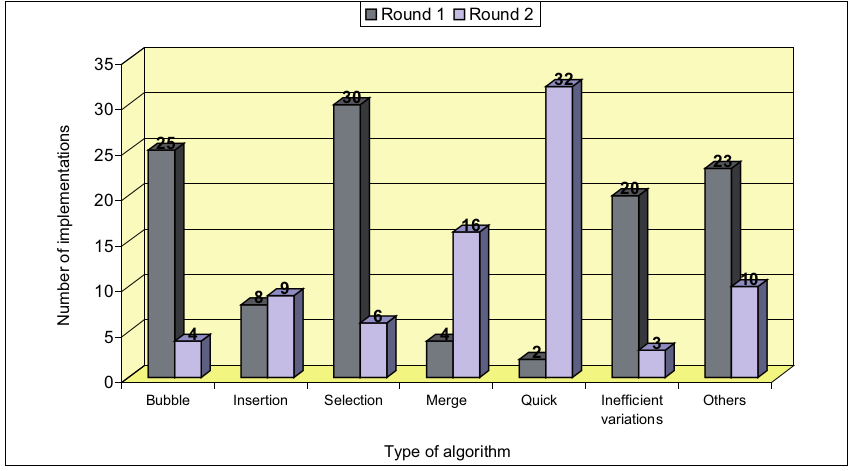
\includegraphics[scale=0.4]{imagem/clusterManual.png}
	        \captionsetup{justification=centering}
	        \caption{Agrupamento manual das implementações dos estudos estudantes na
	        	primeira e segunda etapa}
	        \label{fig:clusterManual}
	    \end{figure}
	    
	    Após o agrupamento manual dos métodos de ordenação implementados pelos alunos,
	    \citeonline{Taherkhani:2012} realizou o reconhecimento automático das
	    implementações por meio da ferramenta Aari. Inicialmente a ferramenta foi
	    treinada para reconhecer os algoritmos de ordenação citados anteriormente.
	    A Figura \ref{fig:clusterAutomatico} apresenta o gráfico para comparar cada
	    agrupamento manual realizado anteriormente com o reconhecimento automático
	    da ferramenta. Possui as mesmas propriedades da Figura \ref{fig:clusterManual}
	    com exceção das colunas. A coluna da esquerda referencia o agrupamento manual
	    de cada algoritmo de ordenação da segunda etapa e a coluna da direita apresenta
	    os algoritmos reconhecidos corretamente pelo Aari. Nota-se que todas as
	    implementações dos métodos de ordenação \foreign{bubble sort},
	    \foreign{selection sort} e \foreign{quicksort} foram classificados corretamente.
	    É possível verificar também que a ferramenta não foi capaz de reconhecer vários
	    algoritmos como \foreign{others}, visto que ele não foi treinado para
	    reconhecer tais algoritmos.
	    
	    \begin{figure}[ht]
	        \centering
	        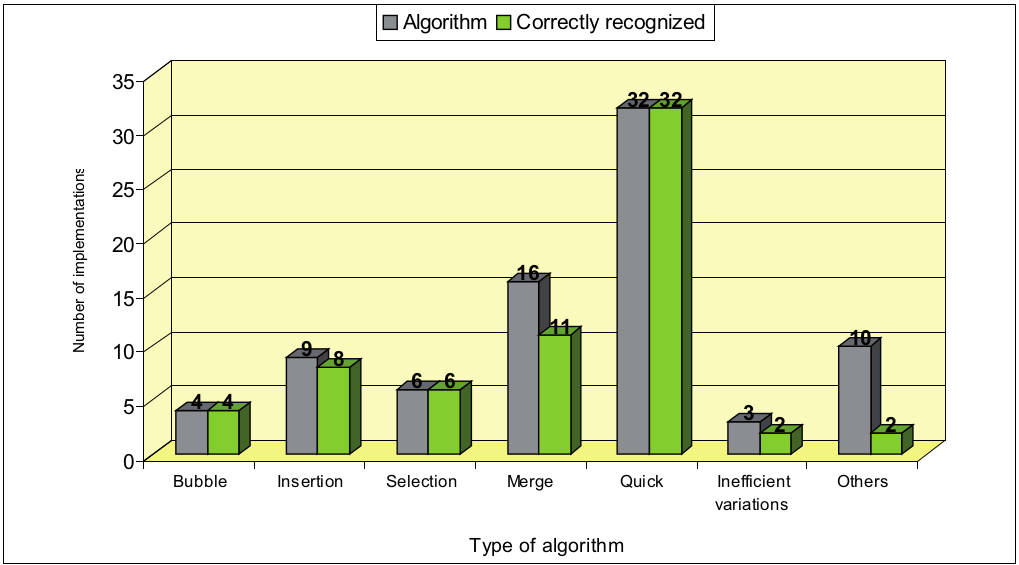
\includegraphics[scale=0.33]{imagem/clusterAutomatico.png}
	        \captionsetup{justification=centering}
	        \caption{Comparação das implementações dos alunos dos \foreign{clusters}
	        	manual e automático da segunda etapa}
	        \label{fig:clusterAutomatico}
	    \end{figure}
	    
	    A ferramenta mostrou-se capaz de identificar a maioria dos métodos de ordenação
	    que foram treinados previamente. Tal abordagem torna-se interessante quando
	    há um plano de ensino com os problemas a serem resolvidos, possibilitando
	    o treinamento da ferramenta. Entretanto, caso seja utilizado para classificar
	    diversos problemas desconhecidos para o classificador, não há uma categorização
	    adequada. Desta forma, inviabilizaria sua utilização em MOOC se fosse utilizado
	    para classificar os problemas de todos os cursos de programação.
	    
	    \citeonline{Glassman:2015} apresentam o OverCode, ferramenta de visualização
	    de informação no qual demonstra os \foreign{clusters} formados, as principais
	    instruções utilizadas pelas implementações presentes em um determinado
	    agrupamento e as linhas de código de uma determinada função/método. A
	    ferramenta é voltada para aqueles que realizarão a validação das submissões.
	    
	    Para verificar a similaridade das submissões a fim de realizar o agrupamento,
	    é necessário: formatar o código-fonte, executar um caso de teste, extrair sequência
	    de variáveis, identificar variáveis em comum, renomear variáveis comuns e únicas
	    para, então, realizar o agrupamento. Formatar o código-fonte consiste na refatoração
	    em cada implementação. Essa refatoração consiste na remoção dos espaços entre os
	    \foreign{tokens}, mantendo os espaços somente após as palavras reservadas, de
	    comentários e de linhas em branco. Essas modificação no código-fonte, além de
	    deixá-lo legível, também permite cada linha de código ser representada como
	    uma \foreign{string} para que seja possível encontrá-lo em outras soluções.
	    
	    A segunda etapa do agrupamento consiste na execução do mesmo caso de teste
	    para todas as implementações. A cada passo da execução, os nomes e valores de
	    variáveis locais e globais, bem como o valor de retorno da função são gravados
	    como se fosse um histórico de execução ou \foreign{trace}. A partir desse
	    histórico, a ferramenta extrai a sequência de valores de todas as variáveis.
	    
	    A partir do conhecimento da sequência de valores de cada variável, o OverCode
	    identifica quais são as variáveis comuns. Tais variáveis são reconhecidas a
	    partir das suas sequências idênticas dado dois ou mais históricos de execução.
	    As variáveis que só ocorrem uma vez no \foreign{trace} são as variáveis únicas.
	    Após reconhecer as variáveis comuns e únicas, a ferramenta renomeia-as para o
	    nome da variável que ocorreu em mais históricos de execução. Após todos esses
	    passos, o agrupamento é realizado por meio de comparação de blocos de código
	    idênticos.
	    
	    \begin{figure}[ht]
	        \centering
	        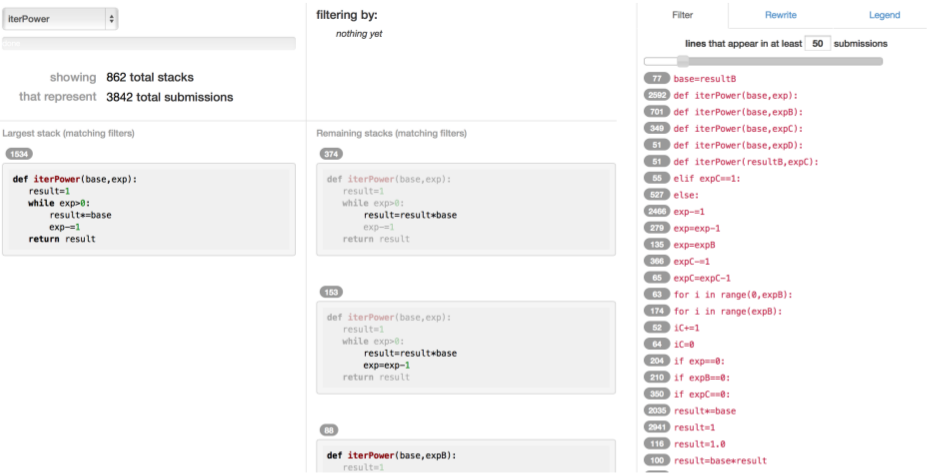
\includegraphics[scale=0.4]{imagem/overCode.png}
	        \captionsetup{justification=centering}
	        \caption{Interface da ferramenta OverCode.}
	        \label{fig:interfaceOverCode}
	    \end{figure}
	    
		Na Figura \ref{fig:interfaceOverCode} é possível notar a utilização das pilhas
		(\foreign{stacks}) para representar os agrupamentos. A primeira coluna da
		esquerda exibe dois painéis. O primeiro painel apresenta o número de
		agrupamentos, representado pelas pilhas, e o número total de submissões,
		enquanto o segundo painel, mostra a maior \foreign{stack}. A coluna central
		apresenta a opção de busca, filtrando por uma determinada palavra no quadro
		superior, e as pilhas remanescentes no quadro inferior. Enquanto a terceira
		coluna apresenta a frequência com que as linhas de códigos estão presentes
		nas soluções das pilhas.

		A comparação das pilhas menores com a pilha maior ocorre entre a primeira e a
	    segunda coluna dando ênfase nas linhas que estão implementadas diferentes. Com
	    isso, é possível verificar como cada pilha foi montada e a característica daquela
	    pilha quando comparada com a pilha maior. Como utiliza análise dinâmica, extraindo
	    o histórico de execução, para agrupar as submissões, é possível verificar o \foreign{trace}
	    da variável que desejar ao longo de sua execução em um caso de teste a fim de
	    auxiliar os usuários a entenderem a execução do algoritmo.

	    Por fim, os autores concluíram que a interface auxilia os assistentes de
	    ensino a terem uma visão de alto nível dos alunos, podendo compreender os
	    erros e fornecer um \foreign{feedback} mais relevante, devido ao agrupamento
	    das implementações, visto que diminui consideravelmente a quantidade de
	    submissões a serem corrigidos.
	    
	    \textbf{Professor, no final do OverCode possui um gráfico interessante relacionando
	    	a quantidade de agrupamentos com o tamanho desses agrupamentos. Entretanto, se
	    	eu utilizar a imagem, acredito que ficaria um pouco poluído essa página, devido
	    	a figura da ferramenta. O gráfico está no repositório: OverCodeDistri.png. A
	    	utilização do gráfico deixaria a minha análise mais fundamentada também.}
	    
	    A divisão das implementações pode ter aumentado consideravelmente o número de
	    agrupamentos. Contudo, a análise dinâmica e os recursos realizados para que
	    fosse montado a pilha mostrou-se eficiente. Todavia, poderia ter considerado
	    toda a implementação e levado em consideração mais uma característica, o tamanho
	    médio das instruções por linha. Devido a diversas possibilidades de realizar
	    uma atribuição com alguma operação aritmética.
	    
	    \citeonline{Wei2015} apresentam uma ferramenta para auxiliar na correção das
	    submissões dos MOOC's de forma a agrupar pedaços (\foreign{chuncks}) de códigos
	    fontes semelhantes, agrupá-los conforme sua similaridade e alocar cada conjunto
	    de implementações ao estudante com conhecimento suficiente para revisá-los.
	    
	    Foi necessário realizar o particionamento do código para torná-lo legível
	    e fácil de compreender. Os pedaços foram extraídos das implementações como
	    se fossem funções. Entretanto, há uma dificuldade para verificar as submissões
	    quando ocorria uma chamada de função em uma outra função, dificultando a divisão
	    em pedaços do código. Também foi necessário normalizar cada submissão a fim de
	    encontrar o estilo de escrita, visto que até mesmo o nome da variável pode
	    alterar o estilo de escrita.
	    
	    A ferramenta desenvolvida por \citeonline{Wei2015} normaliza o código por
	    meio de três regras:
	    
	    \begin{enumerate}
	    	\item Remoção de espaços, linhas em branco e comentários;
	    	\item Exclusão de palavras reservadas da linguagem de programação,
	    	identificadores predefinidos e nomes de funções de bibliotecas;
	    	\item E substituição dos identificadores de variáveis do usuário por um
	    	símbolo especial.
	    \end{enumerate}
	    
	    Com isso foi calculado um valor \foreign{hash},representando cada \foreign{substring}
	    de um código-fonte, a fim de verificar a similaridade do estilo de escrita \foreign{token}
	    a \foreign{token} e utilizado o algoritmo de \texttt{winnowing} \cite{schleimer2003}
	    para escolher o menor subconjunto do estilo de escrita a fim de realizar as
	    comparações por meio do coeficiente de similaridade de \foreign{Jaccard} \cite{jaccard1901}. E
	    com a finalidade de identificar a dificuldade da implementação, foi utilizado
	    a distância Euclidiana para comparar as características extraídas -- quantidade
	    de métodos invocados e laços de repetição aninhados -- e o \foreign{K Nearest Neighbor}
	    (\texttt{k-NN}) para identificar o nível de dificuldade de revisão do
	    \foreign{chunck}.
	    
		\begin{figure}
			\centering
			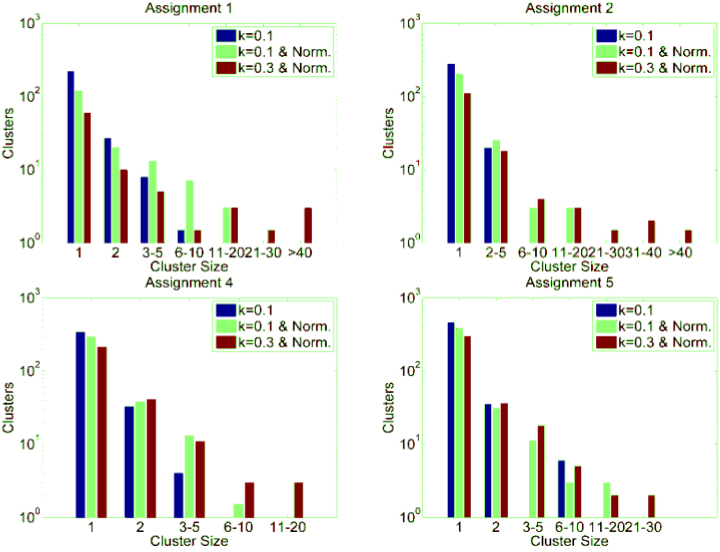
\includegraphics[width=0.7\linewidth]{imagem/clusteringPerformance}
			\captionsetup{justification=centering}
			\caption{Distribuição dos agrupamentos.}
			\label{fig:clusteringPerformance}
		\end{figure}
	    
		A Figura \ref{fig:clusteringPerformance} apresenta a distribuição dos
		agrupamentos em quatro problemas distintos. Para todos os gráficos, a
		abcissa é referente ao tamanho dos pedaços, enquanto a ordenada representa
		o número de agrupamentos. É possível notar três tipos de agrupamento. A barra
		horizontal azul representa o agrupamento sem normalização. enquanto as barras
		verde e vermelho possuem o valor de $k$ diferente, entretanto, ambas estão
		normalizadas. Enquanto a tarefa 1 e 2 apresentou bons agrupamentos e o tamanho
		dos grupos era condizente com a quantidade de estudantes (200) quando $k$ era
		igual a 3.0. As tarefas 4 e 5 não foram satisfeitas devido ao total de pedaços
		em um grupo ser próximo de 20 e o restante dos códigos formaram pequenos
		agrupamentos.
		
		Conforme a Figura \ref{fig:clusteringPerformance}, pode-se notar que a
		distribuição dos \foreign{chuncks} sem normalização de código é inadequado,
		visto que vários pedaços nas tarefas 2 e 4 estavam sozinhos, e o maior
		agrupamento possuía apenas 3 pedaços. Enquanto a tarefa 1 e 2 apresentou
		bons agrupamentos e o tamanho dos grupos era condizente com a quantidade de
		estudantes (200) quando $k$ era igual a 3.0. As tarefas 4 e 5 não foram
		satisfeitas devido ao total de pedaços em um grupo ser próximo de 20 e o
		restante dos códigos foram pequenos agrupamentos.
		
		É possível notar que tal abordagem não obteve sucesso, pois, independente da
		tarefa selecionada, nota-se que a maioria dos \foreign{clusters} formados
		possuíam apenas um pedaço de código. Com isso pode-se aumentar o tempo de
		correção das submissões, visto que uma implementação completa pode gerar um
		ou mais pedaços de código, dificultando a revisão da submissão e podendo tomar
		um tempo maior para que fosse realizado um \foreign{feedback} preciso para o
		estudante.
		
%		\begin{table}
%			\begin{tabular}{|c|c|c|c|c|c|c|}
%				\hline
%				~ & Dados de entrada & Característica extraídas dos dados de entrada & Algoritmo para cálculo de distância ou similariedade & Algoritmo de clusterização / Classificador & Avaliação & Conclusões \\ \hline
%				\citeonline{Yin:2015} & Implementações & AST & Distância de Edição de Árvore (TED) normalizada que utiliza estrutura top-down e pontuação silhueta & DBSCAN e OPTICS & Clusterização de algoritmos baseado nas soluções de um problema. Em cada cluster, identifica as diferenças nas implementações de uma abordagem particular & TED normalizado demonstra conjuntos mais estáveis e menos discrepantes \\ \hline
%				\citeonline{Glassman:2014} & Implementações & Linguagem de alto nível: 12 características - posição de declarações condicionais em relação a instruções de \foreign{loop}, profunidade dos \foreign{loops} aninhados, números de nós AST, instruções de retorno, laços, comparações, etc. Linguagem de baixo nível: 48 características - operações aritméticas, comparações, \foreign{loops}, funções de bibliotecas, declarações, número de variáveis do programa, valores constantes, etc. & ~ & K-means & Utilizando a métrica AMI (\foreign{adjusted mutual information}), comparando os \foreign{cluters} dos feitos pelos professores, no qual 0 indica agrupamentos puramente independentes e 1, perfeita concordância entre os agrupamentos. & Para k maior ou igual a 15, encontrou-se alta concordância entre os \foreign{cluster} do K-means e do professor \\ \hline
%				\citeonline{Taherkhani:2012} & Implementações & Características numéricas: NAS, LoC, MCC, N1, N2, n1, n2, N, n, Nov, NoL, NoNL, NoB. Características descritivas: recursivo, \foreign{tail recursive}, funções de variáveis, \foreign{array} auxiliar. Outras características: informações de \foreign{loop}/bloco, informações do contador de laço, informações de dependência. \foreign{Caracterísitcas} de algoritmos de ordenação: MWH, TEMP, In-place, OIID e IITO. & Vetor de características, calculada a partir das características extraídas das implementações & C4.5 (árvore de decisão) & Com os algoritmos da primeira rodada, obteve 71\% de precisão; da segunda rodada, 81\%. & Bom reconhecimento do algoritmo, se estiver conforme a teoria. Taxa de acerto considerável baseado em um possível erro do professor. Utilização semiautomática: o Aari corrige partes do trabalho no qual foi treinado e o professor, o restante \\ \hline
%				\citeonline{Glassman:2015} & Implementações & Rastro do programa (Sequência de variáveis, variáveis comuns e renomeação de variáveis: colisão comum / comum; colisão de múltiplas instâncias; e colisão único/comum), blocos de código & Comparação de programas bloco a bloco (algoritmo definido no artigo) & Algoritmo definido no artigo (programas iguais na mesma pilha) & No primeiro teste, o \foreign{selection} e o \foreign{insertion sort} foram os mais implementados e, entre todas as implementações, a maioria foi categorizado como "Método próprio". Após a apresentação da matérias aos alunos, um segundo teste foi realizado, assim alguns alunos realizaram a mesma implementação, enquanto outros otimizaram suas implementações em base nos materiais e outros fizeram outros métodos de ordenação & A partir do OverCode e as pilhas com os algoritmos divididos pelas características extraídas, dá a possibilidade de retornar um \foreign{feedback} mais preciso para cada grupo e facilita a observação da solução do problema \\ \hline
%				\citeonline{Wei2015} & Implementações & Normaliza o código e considera apenas o estilo de escrita do estudante & Coeficiente de similaridade de Jaccard & Algoritmo Winnowing & Classificação de \foreign{workload}: distância Euclidiana e k-NN & A classificação por pedaços de código aumentou a eficiência do classificador \\
%				\hline
%			\end{tabular}
%		\end{table}